\section{Deep Space Communications}
\label{sec:space}

There are significant differences between space-based communications and traditional communications on Earth, the physical properties of deep space are fundamental to understand this differences. This section gives a summary of the principal components of space communications and a security overview of current space mission systems. 

%\textbf{Donde poner esto:}
%In traditional networks, the purpose of routing is to select the best path between a source a destination. Routing protocols utilise the network state to calculate the best path according to one or more metrics assuming an almost real-time knowledge of the topology. In space DTNs, the topology could change faster than the time it takes the dissemination of topology updates. Routing still consists of selecting the next best hop until the destination, but the concept of best path is constrained. In this case, maximise the probability of bundle delivery could be the goal \cite{ivancic2009security,fall2003delay,araniti2015contact}. 


\subsection{Space-based communications}

The launch of the Sputnik 1 satellite in 1957 gave origin to the Space Race. Human spaceflights and unmanned robotic space probes were developed to support space exploration. Communication systems were designed to send commands from a mission control centre (telecommand) and receive telemetry or science data from spacecraft. The original idea was simple: the mission control centre sends a radio frequency signal to a spacecraft, then the spacecraft receives the signal via its antenna and process the telecommand. Finally, the spacecraft replies with telemetry commands or science data if requested to do so. Figure \ref{fig:space-based-arc} shows a simplified diagram of space missions architecture.  

%As exploration mission went farther away in the solar system or requiere more science data from spacecraft, communication systems had to evolve to keep the pace of space missions complexity.


\begin{figure}[hbt]
\centering
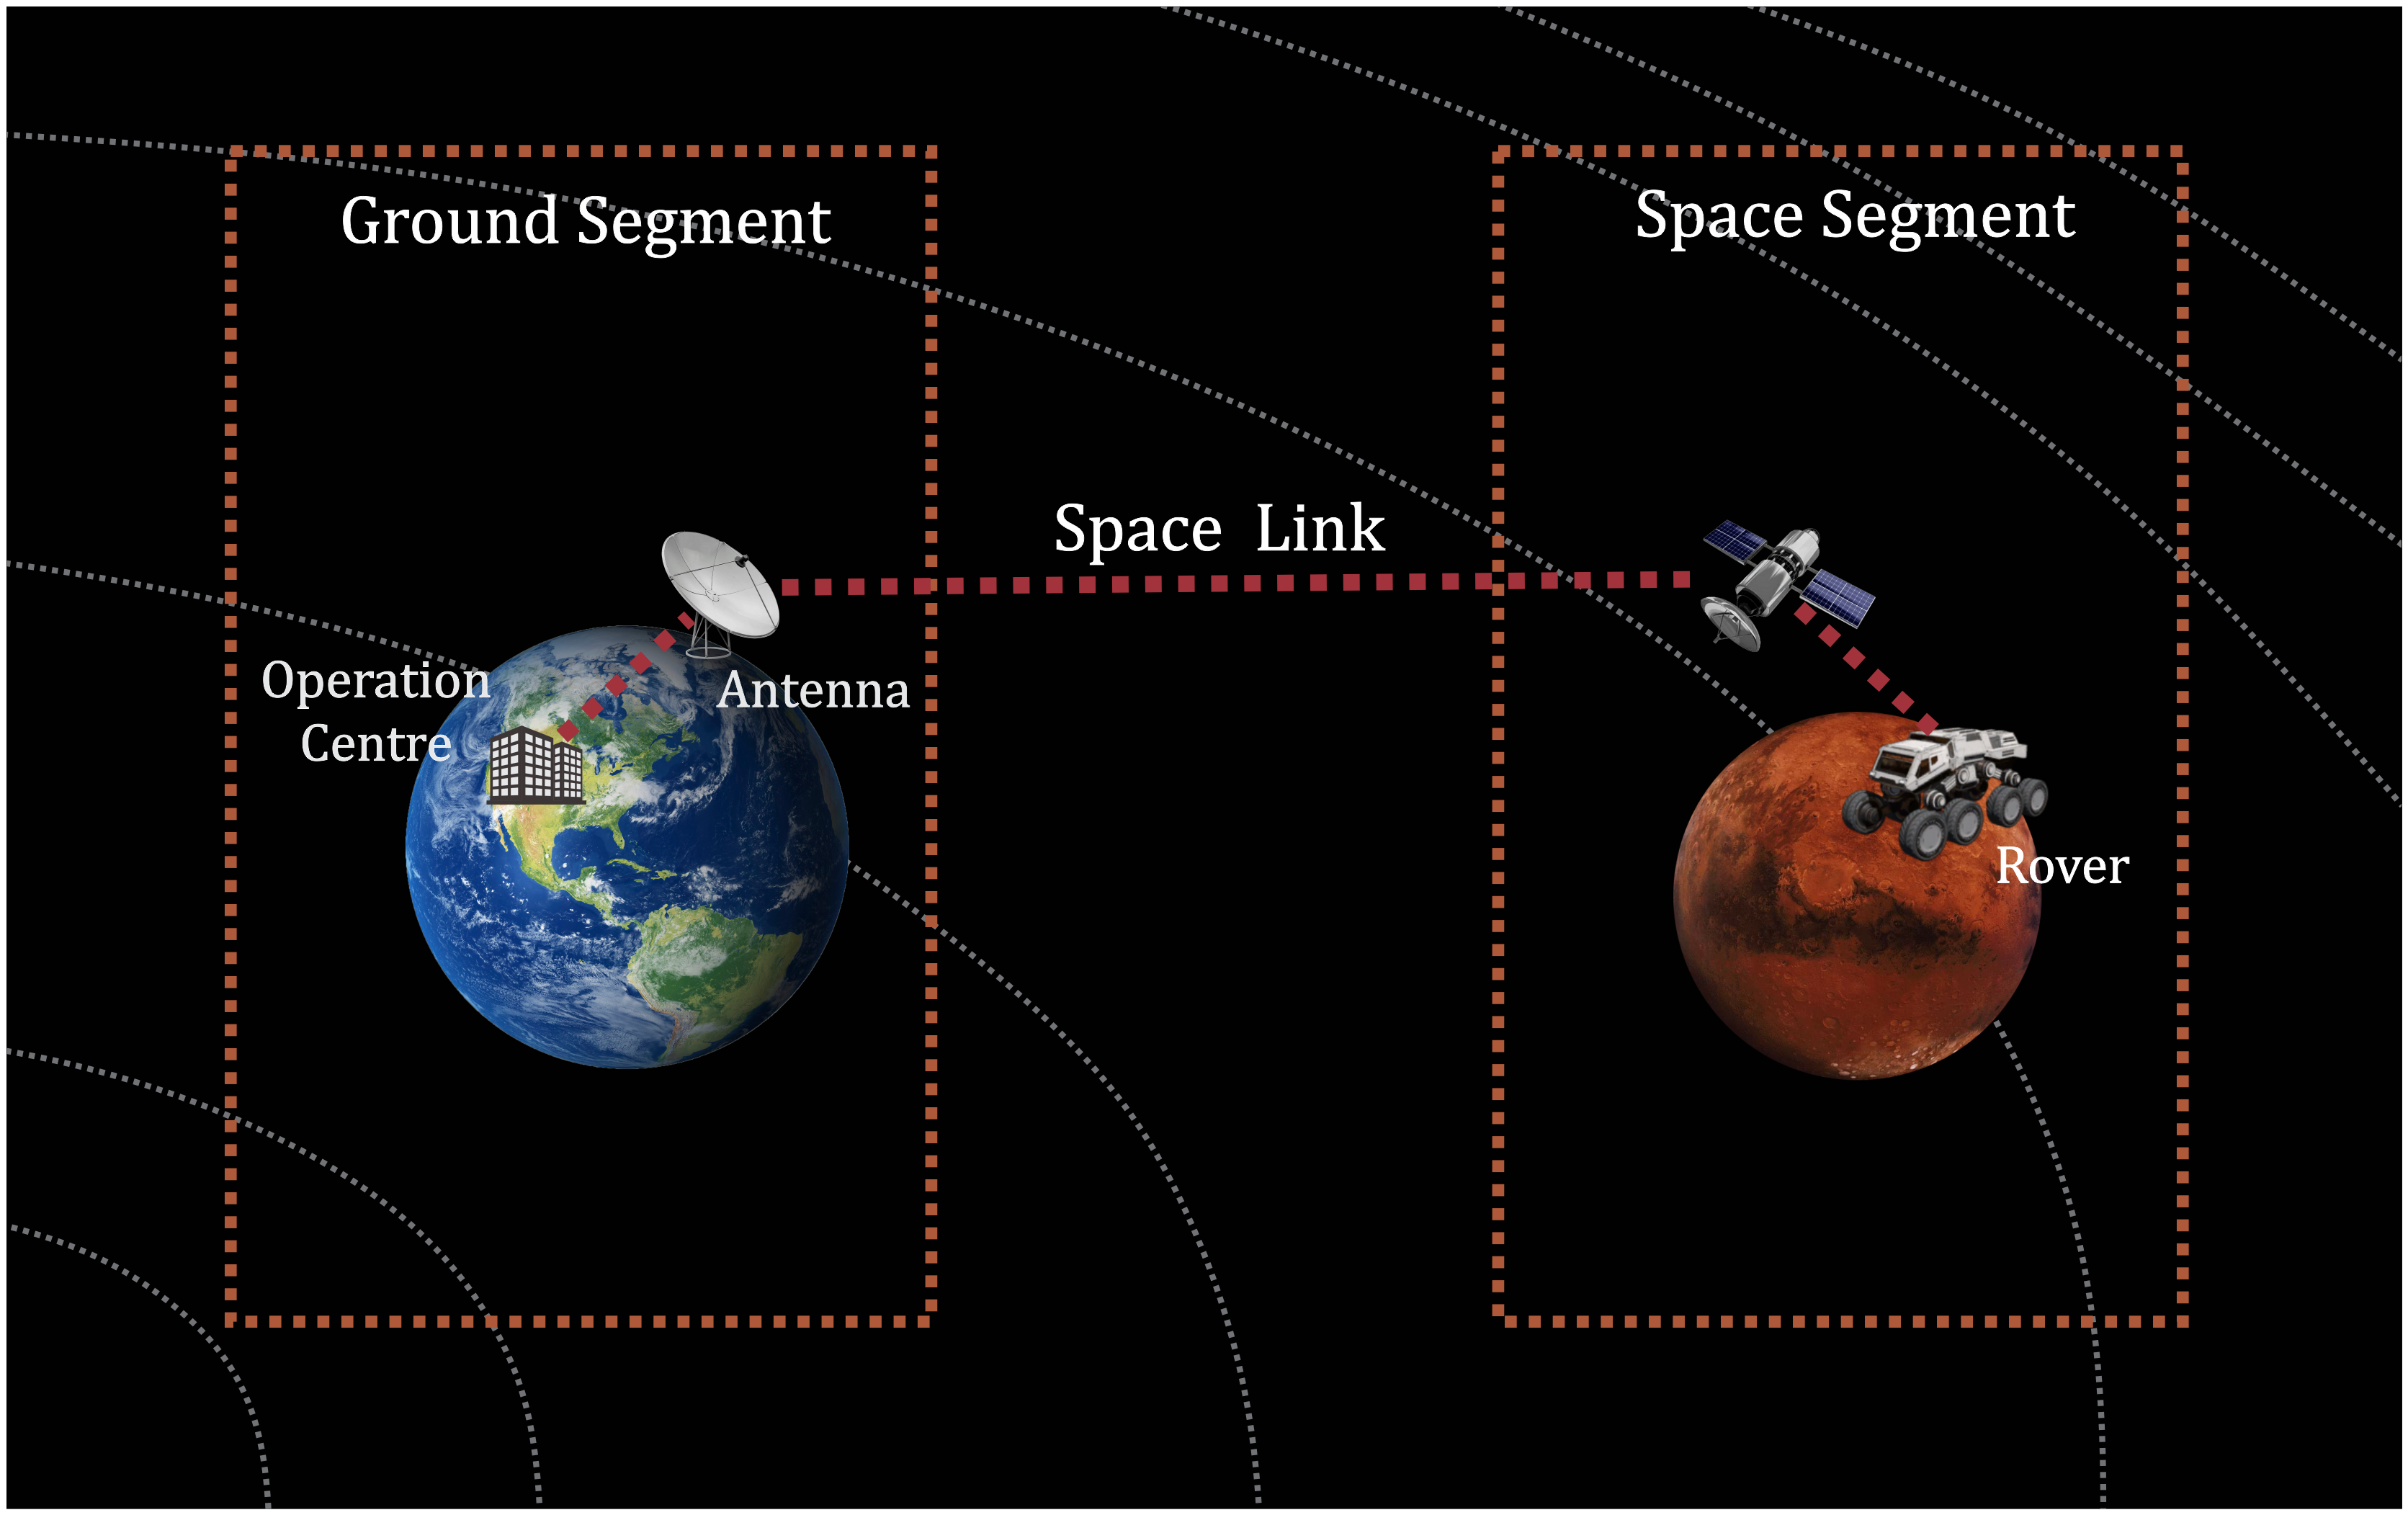
\includegraphics[width=1 \linewidth]{images/ground.png} 
\caption{Space-based communication architecture}
\label{fig:space-based-arc}
\end{figure}

In this example, the satellite and the Mars rover form part of the space segment. The space-link is the connection between the ground station and the satellite.  The ground station and the mission control centre constitute the ground segment. The mission control centre, sometimes called Operational Control Centre (OCC), has the control of the objects in deep space. This example shows the most complex scenario which is currently deployed in the Mars Exploration Rover mission \cite{crisp2003mars}. In the vast majority of space missions, the communication is directly between the OCC and the end-point in the outer space.

 The most significant differences between space-based and terrestrial communications are the long propagation delays due to the speed of light and the lack of end-to-end connectivity caused by planets motion. The result is disrupted communication subject to significant propagation delays. These inherent space properties make well-known protocols for terrestrial networks unsuitable for space communications \cite{fall2003delay}.


The distance of a space object to the Earth determines the type of the communication. Near-earth communications present low delay and intermittent connectivity. Satellites in geosynchronous orbit are subject to low delay but continuous connectivity. Earth-Moon communication is a particular case, the round-trip delay is approximately 2.5 seconds, and there is a disruption in the communication due to the motion of the Earth and the Moon. Space missions beyond the Moon present the worst case: extremely long propagation delay and disrupted communication. For instance,  a signal from the farthest human-made object in deep space (Voyager 1) takes over 19 hours to reach the Earth. Signals sent by Mars rovers take between 7 and 20 minutes to reach Earth, depending on the position of the planets. 
% Moreover, a rover has to be in line-of-sight of an orbiter or the Earth to send or receive data, producing disrupted communication  



Physical limitations are not the only problem; the communication model presents problems as well. Firstly,  the communication infrastructure was designed to be point-to-point. Secondly, each mission operates independently and the cooperation between missions is almost nonexistent. Many missions use bespoke communication protocols and subsequent missions have to ``reinvent the wheel'' \cite{burleigh2003interplanetary}. 

Over the last years the situation is changing, there is an effort from CCSDS and other bodies like IETF to standardise communication protocols for space missions, and space missions started to adopt the new protocols \cite{weber2006transforming}. Examples include Space Packet Protocol (CCSDS), the Bundle Protocol \cite{standard2010ccsds}, and the Licklider Protocol\cite{birrane-dtn-adm-ltp-00}.  % . 

The relay mechanism employed in the Mars Exploration Rover Mission was the first advance towards a packet-switched network style; although, there is no proper inter-networking yet under this configuration. Mars rovers use available orbiters as intermediate hops, but there is no addressing scheme or proper network layer. These limitations will restrict operations of future missions which will require more communication capabilities \cite{rationale2010requirements}. 


The experience in Mars has shown the advantages of multi-hop communication over point-to-point communication. For instance increase in science data return, lower power and hardware requirements, and more contact opportunities \cite{rationale2010requirements}.  Besides, interoperability and cross-support across space agencies will be the usual situation in future space missions. Spacecraft, satellites, rovers and other human-made objects will operate as a network of space-based entities, similar to the figure \ref{fig:inter-internet}. 



\begin{figure}[ht]
\centering
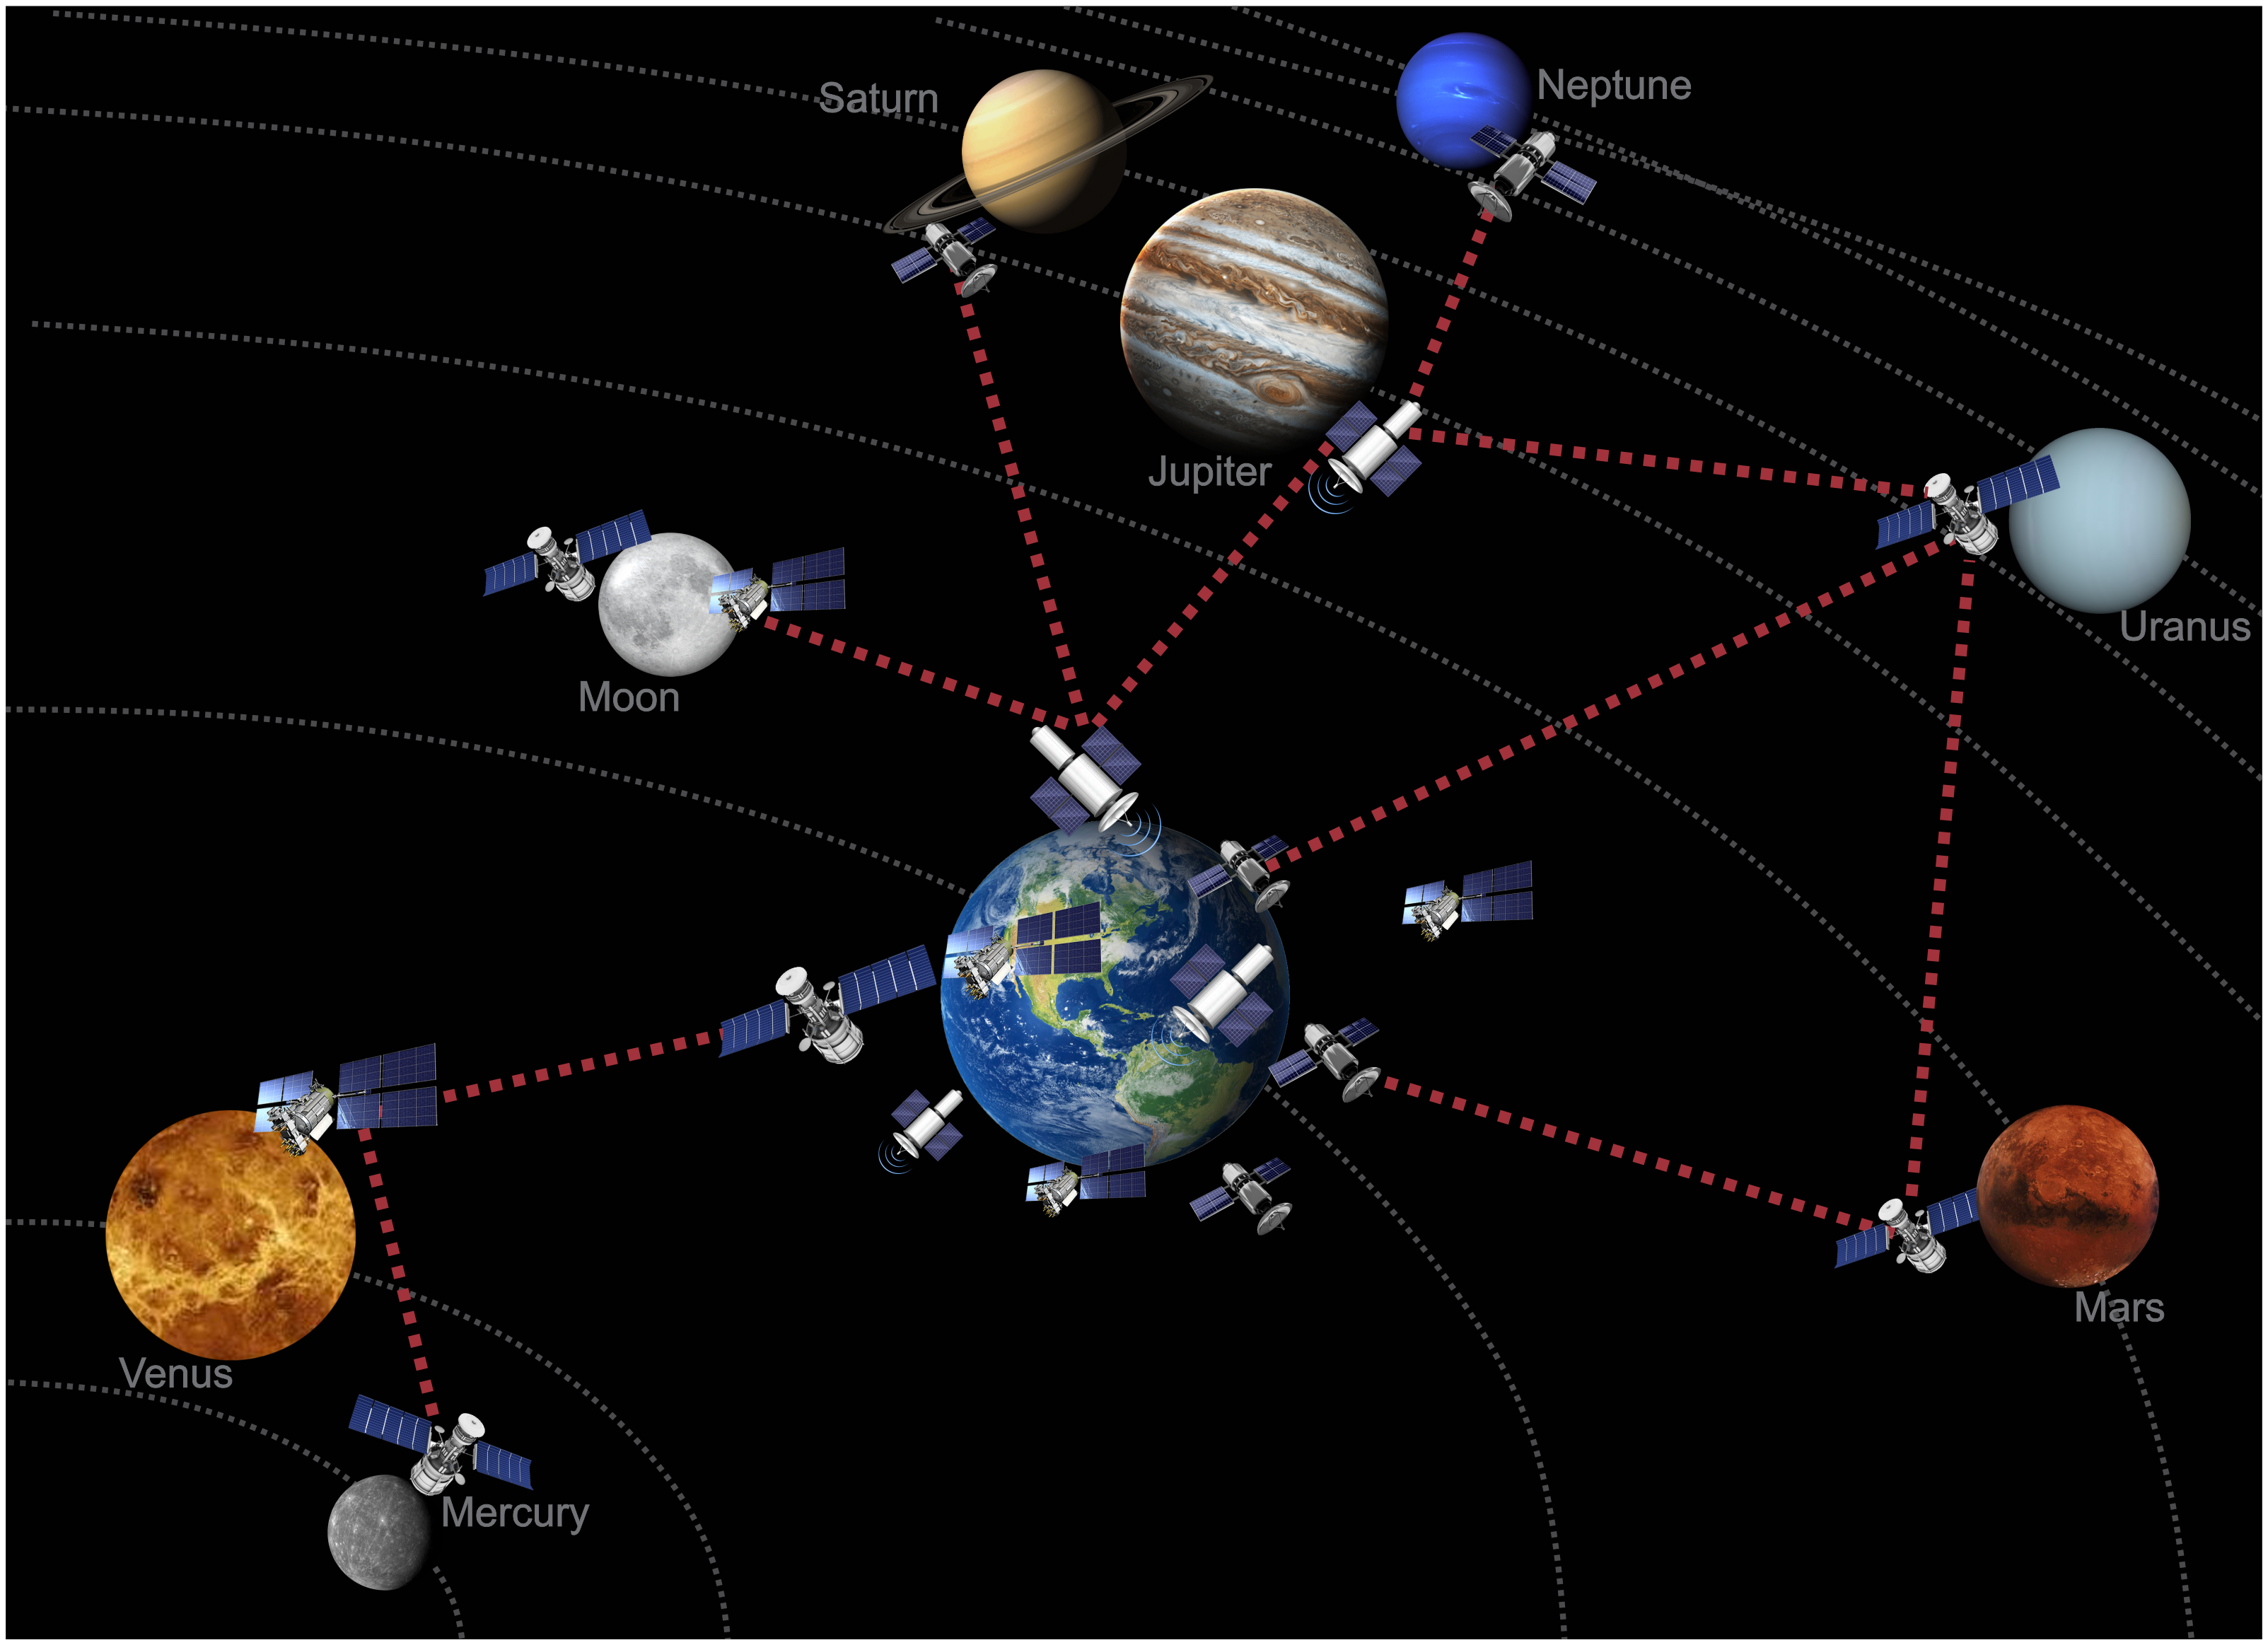
\includegraphics[width=1 \linewidth]{images/interplanetary.png} 
\caption{Interplanetary Internet}
\label{fig:inter-internet}
\end{figure}


\subsection{Security in Space Communications}


Cyber threats apply to all kinds of information systems, especially the ones administrated by nation-states. Space systems are becoming more interconnected to terrestrial networks, and space missions are now target of malicious attackers.  In the past, only military missions were highly protected, but nowadays all types of missions require a certain level of security \cite{book2006security}.

Threats could apply to any segment of space missions, either the space segment, ground segment or space-link. The figure \ref{fig:space-based-arc} illustrates two important points which affect the overall security.  Firstly, the mission control centre and the ground station are not in the same physical location, and the link between them requires a secure connection, consequently key management. Secondly, the network infrastructure on the earth could belong to one entity and the mission control centre to another.  For instance, the  Mars Exploration Mission operates Mars rovers, but the Deep Space Network controls Earth-Mars communications.

Point-to-point space links have been secured using bulk encryption \cite{book2011space}. Although this type of encryption is simple, it requires special techniques and hardware on both ends of the space-link. The problem is that bulk encryption is not suitable for multi-hop communication and interoperability among space agencies. This problem excludes bulk encryption as an option for the Interplanetary Internet. %Ivancic \cite{ivancic2009security} mention potential problem in the US for international interoperability because The International Traffic in Arms Regulations might have jurisdiction.

The CCSDS report considers terrorist, criminals, foreign intelligence services, computer hackers, and commercial competitors as potential adversaries for space missions \cite{book2006security}.  Also, the document states that mission planners must consider security for space systems in the same way as any other information system, as they are subject to passive and active threats. Examples of active threats are jamming, unauthorised access, masquerading, and Denial of Services (DoS); while traffic analysis is considered a passive threat. 

 

% This situation suggests that security for the Interplanetary Internet should consider interoperability not only between nodes from different agencies, but it should consider interoperability between the Internet and space segment protocols. 

 %In \cite{book2012architecture}, CCSDS present security requirements for five space mission profile. These profiles are human spaceflight, earth observation, communication, scientific, and navigation. For instance, humans spaceflights present all security requirements but also ``safety-of-life'' and privacy issues. The security of earth observation, navigation, and communications missions vary depending on the information value and the relative position to the earth. Some missions require security for telemetry, telecommands, and payload communication, others only need to secure a subset of those. 
 
 %These profiles are human spaceflight, earth observation, communication, scientific, and navigation. 
 
Space missions present different mission profiles: human space missions, earth observation satellites, communication satellites, science missions, and navigation satellites \cite{book2012architecture}. Some of them require security for telemetry, telecommands, and payload communication; others only need to secure a subset of those. 


Human spaceflights are especially sensitive, as they require ``safety-of-life'' guarantees. For many countries, satellites already form part of critical infrastructures like navigation, weather study, and disaster response \cite{book2006security}. Science missions present the most challenging scenario. Spacecraft might explore remote locations in the solar system and mission lifetime tend to be extensive. In multi-organisational missions, hardware, payloads and data may belong to different organisations. For multi-hop communication, relay satellites and spacecraft might be administrated by different entities.


As stated before, future missions will require interoperability between space nodes that might be administrated by different agencies. Therefore, space mission planners must consider the implementation of secure communication protocols whether the nodes are in orbit around Earth or exploring remote places in the solar system.


 
 %For instance, humans spaceflights present all security requirements but also ``safety-of-life'' and privacy issues. The security of earth observation, navigation, and communications missions vary depending on the information value and the relative position to the earth. 
 
 %Science missions are more complicated than the previous,  the distance to the earth change requirements dramatically. For interplanetary missions, there are extra factors that should be considered at the time of implementing security, for instance, communication delay, discontinuous communication, fault tolerance, ability to use intermediate nodes (planned and unplanned), significant mission lifetime. The last point to consider is 
 
 %A clear example is optical communications in space, state of the art techniques are not competitive in mass and power performance against radio frequency RF communication, and there are several projects ongoing to meet the performance goals required by mission planners. It remains to see how different profiles could fit in a single key management scheme.
 



\subsection{Key Management in current Missions}

In current space missions, key management complexity is low. Typically, the entities involved are the mission control centre and the spacecraft. The mission control centre is responsible for generating, managing and revoking keys. For human-crewed missions, the human intervention in key management operations is limited. Optionally, the ground station could take part in key management operations if it is working as a security gateway. User facilities may get involved if payload data have to be distributed \cite{book2011space}. 


Commonly keys are stored in smart cards in physical protected places and key generation procedure affects only the ground segment. Master keys are used to generate or exchange new keys of lower hierarchy such as traffic protection keys or key encryption keys. In the case that a master key is used as an encryption key, all key management operations are conducted before launch. Any number of master keys could be used at the discretion of mission planners \cite{book2011space}.

In addition to long delays and disrupted communications, many environmental properties influence communications in space missions, such as asymmetric channels, bandwidth restriction, and remote locations. All these constraints apply to communication and cryptographic protocols, but limited computational resources and memory play a big role for key management. For instance, rovers or sensors might not be able to perform heavy cryptographic operations, and the memory size limits the information that these space objects could store like keys or revocation list.

These limitations imply that symmetric key cryptosystems are more suitable for current space missions \cite{book2011space}, but future space missions present a different scenario, and it is unlikely than symmetric key based cryptosystems will meet the requirements of the Interplanetary Internet.

%It is likely to have group key management for multicast within the network.  

